%==================== Appendix ====================

% This appendix corresponds one-to-one with Chapter 4 in the main text:
% Section A gives proofs of model properties, Section B gives the expressivity analysis,
% Section C gives proofs for the optimization subproblem, and Section D collects supplementary experimental figures.

\section{Basic Model Properties of NTD-PL}
\label{app:model_properties}

This section corresponds to Section~4.3 of the main text and gathers supplementary proofs for the model-family relations, parameter complexity, and scale indeterminacy of NTD-PL. The main text retains only the statements and their meanings, while the detailed derivations are collected here.

\subsection{Reduction to Tucker and Nested Model Families}

\begin{proposition}[Reduction to Tucker]
\label{prop:tucker_special_case_app}
If $\beta_1=1$ and $\beta_p=0$ for all $p\neq 1$, then \eqref{eq:ntdpl_model} reduces to the standard Tucker model, namely
\begin{equation}
\widehat{\cY}
=
\cS
=
\llbracket \cX;\mathbf A^{(1)},\dots,\mathbf A^{(N)}\rrbracket.
\end{equation}
\end{proposition}

\begin{proof}
By the definition of NTD-PL,
\begin{equation}
\widehat{\cY}
=
\sum_{p=0}^{P}\beta_p \cS^{\odot p},
\end{equation}
and when $\beta_1=1$ and $\beta_p=0$ for $p\neq 1$, the above expression reduces to
\begin{equation}
\widehat{\cY}
=
\cS.
\end{equation}
Since $\cS=\llbracket \cX;\mathbf A^{(1)},\dots,\mathbf A^{(N)}\rrbracket$, we recover the standard Tucker decomposition form.
\end{proof}

\begin{proposition}[Degree Nesting]
\label{prop:nested_model_family_app}
For any $P_1<P_2$, the degree-$P_1$ NTD-PL model class is a subset of the degree-$P_2$ model class.
\end{proposition}

\begin{proof}
Take any degree-$P_1$ NTD-PL model,
\begin{equation}
\widehat{\cY}
=
\sum_{p=0}^{P_1}\beta_p \cS^{\odot p}.
\end{equation}
If we view it as a degree-$P_2$ model, it suffices to set
\begin{equation}
\beta_p=0,\qquad p=P_1+1,\dots,P_2,
\end{equation}
to obtain exactly the same output. Therefore, every degree-$P_1$ model belongs to the degree-$P_2$ model class.
\end{proof}

\subsection{Parameter Complexity}

\begin{proposition}[Parameter Complexity]
\label{prop:param_complexity_app}
Let the Tucker multilinear rank be $(R_1,\dots,R_N)$. Then the total number of parameters in NTD-PL is
\begin{equation}
\#\mathrm{param}
=
\prod_{n=1}^{N}R_n
+
\sum_{n=1}^{N}I_nR_n
+
(P+1).
\end{equation}
\end{proposition}

\begin{proof}
The parameters of NTD-PL consist of three parts:

\begin{enumerate}
    \item The core tensor $\cX\in\mathbb{R}^{R_1\times\cdots\times R_N}$, whose number of parameters is
    \begin{equation}
    \prod_{n=1}^{N}R_n;
    \end{equation}

    \item The mode factor matrices $\mathbf A^{(n)}\in\mathbb{R}^{I_n\times R_n}$, whose total number of parameters is
    \begin{equation}
    \sum_{n=1}^{N}I_nR_n;
    \end{equation}

    \item The polynomial link coefficients $\boldsymbol\beta=(\beta_0,\beta_1,\dots,\beta_P)^\top$, whose number of parameters is
    \begin{equation}
    P+1.
    \end{equation}
\end{enumerate}

Adding the three parts together gives
\begin{equation}
\#\mathrm{param}
=
\prod_{n=1}^{N}R_n
+
\sum_{n=1}^{N}I_nR_n
+
(P+1).
\end{equation}
\end{proof}

\subsection{Scale Indeterminacy and the Normalization Mechanism}

We now show that NTD-PL inherits the scale indeterminacy of Tucker decomposition. Therefore, the normalization step in the main text should be understood as a gauge-fixing mechanism rather than as an additional constraint that changes the model class.

\begin{proposition}[Scale Invariance]
\label{prop:scale_invariance_app}
Let
\begin{equation}
\cS
=
\llbracket \cX;\mathbf A^{(1)},\dots,\mathbf A^{(N)}\rrbracket.
\end{equation}
For a given mode $n$, take any invertible diagonal matrix $D^{(n)}\in\mathbb{R}^{R_n\times R_n}$ and define
\begin{equation}
\widetilde{\mathbf A}^{(n)} = \mathbf A^{(n)}D^{(n)},\qquad
\widetilde{\cX} = \cX \times_n (D^{(n)})^{-1}.
\end{equation}
Then
\begin{equation}
\llbracket \widetilde{\cX};\mathbf A^{(1)},\dots,\mathbf A^{(n-1)},\widetilde{\mathbf A}^{(n)},\mathbf A^{(n+1)},\dots,\mathbf A^{(N)}\rrbracket
=
\cS.
\end{equation}
Therefore, for any polynomial coefficients $\boldsymbol\beta$, the NTD-PL output
\begin{equation}
\widehat{\cY}=f_{\boldsymbol\beta}(\cS)
\end{equation}
remains unchanged.
\end{proposition}

\begin{proof}
Using the associativity of mode products in Tucker reconstruction,
\[
(\cX\times_n B)\times_n A = \cX\times_n (AB),
\]
we obtain
\begin{align}
\llbracket \widetilde{\cX};\mathbf A^{(1)},\dots,\widetilde{\mathbf A}^{(n)},\dots,\mathbf A^{(N)}\rrbracket
&=
\widetilde{\cX}\times_1 \mathbf A^{(1)}\times\cdots\times_n \widetilde{\mathbf A}^{(n)}\times\cdots\times_N \mathbf A^{(N)} \\
&=
\bigl(\cX\times_n (D^{(n)})^{-1}\bigr)\times_n \bigl(\mathbf A^{(n)}D^{(n)}\bigr)\times_{m\neq n}\mathbf A^{(m)} \\
&=
\cX\times_n \Bigl(\bigl(\mathbf A^{(n)}D^{(n)}\bigr)(D^{(n)})^{-1}\Bigr)\times_{m\neq n}\mathbf A^{(m)} \\
&=
\cX\times_n \mathbf A^{(n)}\times_{m\neq n}\mathbf A^{(m)} \\
&=
\llbracket \cX;\mathbf A^{(1)},\dots,\mathbf A^{(N)}\rrbracket
=
\cS.
\end{align}
Hence, collinear rescaling together with core absorption does not change the latent tensor $\cS$. Since the output of NTD-PL depends only on $\cS$,
\begin{equation}
\widehat{\cY}
=
f_{\boldsymbol\beta}(\cS)
=
\sum_{p=0}^{P}\beta_p \cS^{\odot p},
\end{equation}
$\widehat{\cY}$ also remains unchanged whenever $\cS$ is unchanged.
\end{proof}

\begin{remark}
Proposition~\ref{prop:scale_invariance_app} shows that column normalization of the factor matrices together with absorbing the scale into the core tensor does not change the output of NTD-PL; it only selects a more stable representative from an equivalence class of parameterizations. Since higher-order terms $\cS^{\odot p}$ are more sensitive to scale, such normalization is particularly important in polynomial-link models.
\end{remark}

\section{Expressivity Analysis Under Element-Wise Nonlinear Generation}
\label{app:expressivity}

This section corresponds to Section~4.3.2 of the main text and gives the basic expressivity results of NTD-PL under an element-wise nonlinear generation model. Consistent with the main text, let the true Tucker latent tensor be
\begin{equation}
\cS^\star
=
\llbracket
\cX^\star;\,
\mathbf A^{(1)\star},\dots,\mathbf A^{(N)\star}
\rrbracket
\in \R^{I_1\times\cdots\times I_N},
\end{equation}
and let the total number of entries be
\begin{equation}
N_e=\prod_{n=1}^N I_n.
\end{equation}
Assume that the observation tensor is generated by applying some scalar function $g:\R\to\R$ element-wise, that is,
\begin{equation}
\cY = g(\cS^\star), \qquad
\cY_{i_1,\dots,i_N}
=
g\!\left(\cS^\star_{i_1,\dots,i_N}\right).
\end{equation}

The NTD-PL model class is written as
\begin{equation}
\widehat{\cY}
=
f_{\boldsymbol\beta}(\cS)
=
\sum_{p=0}^{P}\beta_p \cS^{\odot p},
\qquad
\cS=
\llbracket
\cX;\,
\mathbf A^{(1)},\dots,\mathbf A^{(N)}
\rrbracket,
\label{eq:ntdpl_appendix_model}
\end{equation}
where $\cS^{\odot p}$ denotes the element-wise $p$th power of $\cS$, and $\boldsymbol\beta=(\beta_0,\dots,\beta_P)$ are the polynomial link coefficients.

\begin{assumption}[Boundedness]
\label{ass:bounded_S}
There exists a constant $B>0$ such that
\begin{equation}
\norm{\cS^\star}_{\infty}\le B.
\end{equation}
\end{assumption}

Assumption~\ref{ass:bounded_S} is natural in practice, because data preprocessing and scale normalization in the model usually keep the latent Tucker tensor within a bounded range.

\subsection{Exact Representation Under Polynomial Generation}

\begin{theorem}[Exact Representation Under a Polynomial Link]
\label{thm:poly_exact}
Suppose the true generating function $g$ is a real-coefficient polynomial of degree at most $P$, namely
\begin{equation}
g(x)=\sum_{p=0}^{P} c_p x^p.
\end{equation}
If the true observation tensor satisfies
\begin{equation}
\cY = g(\cS^\star),
\qquad
\cS^\star
=
\llbracket
\cX^\star;\,
\mathbf A^{(1)\star},\dots,\mathbf A^{(N)\star}
\rrbracket,
\end{equation}
then NTD-PL can represent $\cY$ exactly at degree $P$. More specifically, it suffices to take
\begin{equation}
\cX=\cX^\star,\qquad
\mathbf A^{(n)}=\mathbf A^{(n)\star}\ \ (n=1,\dots,N),\qquad
\beta_p=c_p\ \ (p=0,\dots,P),
\end{equation}
in which case
\begin{equation}
\widehat{\cY}
=
\sum_{p=0}^{P}\beta_p (\cS^\star)^{\odot p}
=
g(\cS^\star)
=
\cY.
\end{equation}
\end{theorem}

\begin{proof}
For any index $(i_1,\dots,i_N)$,
\begin{equation}
\widehat{\cY}_{i_1,\dots,i_N}
=
\sum_{p=0}^{P} c_p
\bigl(\cS^\star_{i_1,\dots,i_N}\bigr)^p
=
g\!\left(\cS^\star_{i_1,\dots,i_N}\right)
=
\cY_{i_1,\dots,i_N}.
\end{equation}
Since the equality holds for all entries, we have $\widehat{\cY}=\cY$.
\end{proof}

\begin{corollary}[Exact Recovery Under Polynomial Nonlinearity]
\label{cor:poly_recovery}
If the true generation satisfies
\begin{equation}
\cY=\cS^\star + \alpha\, h(\cS^\star),
\end{equation}
where $h$ is a polynomial of degree at most $d$, then whenever $P\ge d$, there exists a set of NTD-PL parameters such that
\begin{equation}
\widehat{\cY}=\cY.
\end{equation}
\end{corollary}

\begin{proof}
View
\begin{equation}
g(x)=x+\alpha h(x)
\end{equation}
as a polynomial of degree at most $\max\{1,d\}$. If $P\ge d$, then the degree of $g$ is at most $P$, and the conclusion follows directly from Theorem~\ref{thm:poly_exact}.
\end{proof}

\subsection{Approximation Bounds Under General Element-Wise Nonlinearity}

We now show that when the true nonlinear function is not a polynomial, the approximation error of NTD-PL can be controlled by the approximation error of a one-dimensional scalar function.

\begin{theorem}[Tensor Approximation Bound Induced by Scalar Function Approximation]
\label{thm:scalar_to_tensor}
Assume that Assumption~\ref{ass:bounded_S} holds, and let
\begin{equation}
q_P(x)=\sum_{p=0}^{P}\beta_p x^p
\end{equation}
be any polynomial of degree at most $P$. If we take the latent variable of NTD-PL to be the true latent tensor, i.e., $\cS=\cS^\star$, then
\begin{equation}
\norm{
g(\cS^\star)-q_P(\cS^\star)
}_F
\le
\sqrt{N_e}\,
\sup_{|x|\le B}\,
|g(x)-q_P(x)|.
\label{eq:scalar_to_tensor_bound}
\end{equation}
\end{theorem}

\begin{proof}
For any entry $(i_1,\dots,i_N)$, since $\norm{\cS^\star}_\infty\le B$, we have
\begin{equation}
\left|
g\!\left(\cS^\star_{i_1,\dots,i_N}\right)
-
q_P\!\left(\cS^\star_{i_1,\dots,i_N}\right)
\right|
\le
\sup_{|x|\le B}|g(x)-q_P(x)|.
\end{equation}
Squaring both sides and summing over all $N_e$ entries yields
\begin{equation}
\norm{
g(\cS^\star)-q_P(\cS^\star)
}_F^2
\le
N_e\,
\left(
\sup_{|x|\le B}|g(x)-q_P(x)|
\right)^2.
\end{equation}
Taking square roots on both sides gives \eqref{eq:scalar_to_tensor_bound}.
\end{proof}

\begin{remark}
Theorem~\ref{thm:scalar_to_tensor} shows that, when the true latent variable $\cS^\star$ is fixed, the tensor approximation problem of NTD-PL can be reduced to a one-dimensional function approximation problem on the interval $[-B,B]$. Therefore, when the true nonlinearity is an analytic function such as $\sin(\cdot)$ or $\tanh(\cdot)$, the quality of the result is determined by the approximation quality of the corresponding polynomial truncation on that interval.
\end{remark}

\subsection{Explicit Truncation Error Bound for Analytic Functions}

\begin{theorem}[Explicit Truncation Bound for Analytic Link Functions]
\label{thm:analytic_bound}
Suppose that $g$ is analytic on the complex disk
\begin{equation}
D(0,\rho)=\{z\in\mathbb{C}: |z|<\rho\}
\end{equation}
and satisfies
\begin{equation}
0<B<\rho,
\qquad
\norm{\cS^\star}_\infty\le B.
\end{equation}
Let the Taylor expansion of $g$ at $0$ be
\begin{equation}
g(x)=\sum_{p=0}^{\infty} a_p x^p,
\end{equation}
and let its degree-$P$ truncation be
\begin{equation}
q_P(x)=\sum_{p=0}^{P} a_p x^p.
\end{equation}
Define
\begin{equation}
M_\rho=\sup_{|z|=\rho}|g(z)|.
\end{equation}
Then
\begin{equation}
\norm{
g(\cS^\star)-q_P(\cS^\star)
}_F
\le
\sqrt{N_e}\,M_\rho
\frac{(B/\rho)^{P+1}}{1-B/\rho}.
\label{eq:analytic_truncation_bound}
\end{equation}
\end{theorem}

\begin{proof}
By Cauchy's estimate,
\begin{equation}
|a_p|\le \frac{M_\rho}{\rho^p},\qquad p=0,1,2,\dots
\end{equation}
Hence for any $|x|\le B$,
\begin{align}
|g(x)-q_P(x)|
&=
\left|
\sum_{p=P+1}^{\infty} a_p x^p
\right|
\le
\sum_{p=P+1}^{\infty}|a_p||x|^p \\
&\le
M_\rho
\sum_{p=P+1}^{\infty}(B/\rho)^p
=
M_\rho \frac{(B/\rho)^{P+1}}{1-B/\rho}.
\end{align}
Applying Theorem~\ref{thm:scalar_to_tensor} then gives
\begin{equation}
\norm{
g(\cS^\star)-q_P(\cS^\star)
}_F
\le
\sqrt{N_e}\,M_\rho
\frac{(B/\rho)^{P+1}}{1-B/\rho}.
\end{equation}
This completes the proof.
\end{proof}

\begin{remark}
Theorem~\ref{thm:analytic_bound} provides an explicit error bound. It shows that:
\begin{enumerate}
    \item as $P$ increases, if $B<\rho$, then the truncation error decays geometrically with $P$;
    \item for the same degree $P$, approximation becomes more difficult as the amplitude range $B$ of the latent variable grows;
    \item this provides a theoretical explanation for the performance differences observed in the experiments under different nonlinear functions, different nonlinear strengths, and different normalization strategies.
\end{enumerate}
\end{remark}

\subsection{\texorpdfstring{Relation to the Nonlinear Energy-Ratio Parameter $\alpha$}{Relation to the Nonlinear Energy-Ratio Parameter alpha}}
\label{app:alpha_energy_ratio}

In the synthetic data of this paper, the nonlinear-strength parameter $\alpha$ is defined in terms of an \emph{energy ratio}, rather than as a direct coefficient multiplying the nonlinear term. Let the linear base tensor be
\begin{equation}
\cS^\star \in \mathbb{R}^{I_1\times\cdots\times I_N},
\end{equation}
and let
\begin{equation}
\cX^\star = g(\cS^\star)
\end{equation}
denote the tensor obtained after some element-wise nonlinear transformation. To avoid counting the linear component of $\cX^\star$ along $\cS^\star$ twice as part of the nonlinear component, we first define the orthogonalized residual
\begin{equation}
\cR^\star
=
\cX^\star
-
\frac{\langle \cX^\star,\cS^\star\rangle}{\|\cS^\star\|_F^2}\,\cS^\star.
\label{eq:orthogonal_residual_app}
\end{equation}
If $\|\cR^\star\|_F>0$, we further define the normalized residual
\begin{equation}
\widetilde{\cR}^\star
=
\frac{\|\cS^\star\|_F}{\|\cR^\star\|_F}\,\cR^\star.
\label{eq:normalized_residual_app}
\end{equation}
The observation tensor is then constructed as
\begin{equation}
\cY_\alpha
=
\sqrt{1-\alpha}\,\cS^\star
+
\sqrt{\alpha}\,\widetilde{\cR}^\star,
\qquad
0\le \alpha\le 1.
\label{eq:alpha_energy_model_app}
\end{equation}

This construction is consistent with the data-generation procedure used in the implementation: we first remove from the nonlinear transform its projection onto the linear backbone, then rescale the residual to have the same target energy as the original tensor, and finally mix the two components with coefficients $\sqrt{1-\alpha}$ and $\sqrt{\alpha}$ in terms of energy.

\begin{proposition}[Interpretation as an Energy Ratio]
\label{prop:alpha_energy_ratio_app}
Let $\cY_\alpha$ be defined by \eqref{eq:alpha_energy_model_app}, and assume that $\|\cR^\star\|_F>0$. Then
\begin{equation}
\langle \cS^\star,\widetilde{\cR}^\star\rangle = 0,
\qquad
\|\widetilde{\cR}^\star\|_F = \|\cS^\star\|_F,
\end{equation}
hence
\begin{equation}
\|\cY_\alpha\|_F^2=\|\cS^\star\|_F^2,
\label{eq:energy_preserved_app}
\end{equation}
and the energy proportions of the linear and nonlinear parts satisfy
\begin{equation}
\frac{\|\sqrt{1-\alpha}\,\cS^\star\|_F^2}{\|\cY_\alpha\|_F^2}=1-\alpha,
\qquad
\frac{\|\sqrt{\alpha}\,\widetilde{\cR}^\star\|_F^2}{\|\cY_\alpha\|_F^2}=\alpha.
\label{eq:energy_ratio_exact_app}
\end{equation}
\end{proposition}

\begin{proof}
From \eqref{eq:orthogonal_residual_app}, we have
\begin{equation}
\langle \cS^\star,\cR^\star\rangle=0,
\end{equation}
hence
\begin{equation}
\langle \cS^\star,\widetilde{\cR}^\star\rangle=0.
\end{equation}
From \eqref{eq:normalized_residual_app}, we also have
\begin{equation}
\|\widetilde{\cR}^\star\|_F=\|\cS^\star\|_F.
\end{equation}
Therefore,
\begin{align}
\|\cY_\alpha\|_F^2
&=
\left\|
\sqrt{1-\alpha}\,\cS^\star+\sqrt{\alpha}\,\widetilde{\cR}^\star
\right\|_F^2 \\
&=
(1-\alpha)\|\cS^\star\|_F^2
+
\alpha\|\widetilde{\cR}^\star\|_F^2
+
2\sqrt{\alpha(1-\alpha)}
\langle \cS^\star,\widetilde{\cR}^\star\rangle \\
&=
(1-\alpha)\|\cS^\star\|_F^2+\alpha\|\cS^\star\|_F^2 \\
&=
\|\cS^\star\|_F^2,
\end{align}
which gives \eqref{eq:energy_preserved_app}. Computing the proportion of the total energy carried by each part then yields \eqref{eq:energy_ratio_exact_app}.
\end{proof}

We next analyze how the truncation error of NTD-PL varies with $\alpha$ under this energy-ratio definition.

\begin{corollary}[Relation Between Truncation Error and $\alpha$]
\label{cor:alpha_truncation_app}
Suppose
\begin{equation}
\cX^\star = g(\cS^\star),
\qquad
\|\cS^\star\|_\infty \le B,
\end{equation}
and define
\begin{equation}
c_g
=
\frac{\langle \cX^\star,\cS^\star\rangle}{\|\cS^\star\|_F^2},
\qquad
\eta_g
=
\frac{\|\cS^\star\|_F}{\|\cR^\star\|_F},
\end{equation}
where $\cR^\star$ is defined by \eqref{eq:orthogonal_residual_app}. Let $q_P$ be a polynomial approximation to $g$ on the interval $[-B,B]$ of degree at most $P$, satisfying
\begin{equation}
\varepsilon_P(B)
:=
\sup_{|s|\le B}|g(s)-q_P(s)|,
\end{equation}
and define
\begin{equation}
a_\alpha=\sqrt{1-\alpha}-\sqrt{\alpha}\,\eta_g c_g,
\qquad
b_\alpha=\sqrt{\alpha}\,\eta_g.
\end{equation}
Then there exists a corresponding degree-$P$ representation
\begin{equation}
\widehat{\cY}_{\alpha,P}
=
a_\alpha \cS^\star + b_\alpha q_P(\cS^\star),
\end{equation}
such that
\begin{equation}
\|\cY_\alpha-\widehat{\cY}_{\alpha,P}\|_F
\le
\sqrt{\alpha}\,\eta_g\,\sqrt{N_e}\,\varepsilon_P(B),
\label{eq:alpha_truncation_bound_app}
\end{equation}
where
\begin{equation}
N_e=\prod_{n=1}^N I_n.
\end{equation}
Furthermore,
\begin{equation}
\|\cY_\alpha-\widehat{\cY}_{\alpha,P}\|_F^2
\le
\alpha\,\eta_g^2\,N_e\,\varepsilon_P(B)^2.
\label{eq:alpha_truncation_bound_sq_app}
\end{equation}
\end{corollary}

\begin{proof}
From \eqref{eq:orthogonal_residual_app}--\eqref{eq:normalized_residual_app},
\begin{equation}
\widetilde{\cR}^\star
=
\eta_g\bigl(\cX^\star-c_g\cS^\star\bigr)
=
\eta_g\bigl(g(\cS^\star)-c_g\cS^\star\bigr).
\end{equation}
Substituting this into \eqref{eq:alpha_energy_model_app} yields
\begin{align}
\cY_\alpha
&=
\sqrt{1-\alpha}\,\cS^\star
+
\sqrt{\alpha}\,\eta_g\bigl(g(\cS^\star)-c_g\cS^\star\bigr) \\
&=
\bigl(\sqrt{1-\alpha}-\sqrt{\alpha}\,\eta_g c_g\bigr)\cS^\star
+
\sqrt{\alpha}\,\eta_g\,g(\cS^\star) \\
&=
a_\alpha \cS^\star + b_\alpha g(\cS^\star).
\end{align}
Hence
\begin{equation}
\cY_\alpha-\widehat{\cY}_{\alpha,P}
=
b_\alpha\bigl(g(\cS^\star)-q_P(\cS^\star)\bigr).
\end{equation}
Using $|b_\alpha|=\sqrt{\alpha}\,\eta_g$ together with
\begin{equation}
\|g(\cS^\star)-q_P(\cS^\star)\|_F
\le
\sqrt{N_e}\,\varepsilon_P(B),
\end{equation}
we obtain
\begin{equation}
\|\cY_\alpha-\widehat{\cY}_{\alpha,P}\|_F
\le
\sqrt{\alpha}\,\eta_g\,\sqrt{N_e}\,\varepsilon_P(B).
\end{equation}
Squaring both sides gives \eqref{eq:alpha_truncation_bound_sq_app}.
\end{proof}

\begin{remark}
Corollary~\ref{cor:alpha_truncation_app} shows that under the energy-ratio generation mechanism adopted in this paper:

\begin{enumerate}
    \item the upper bound of the truncation error in Frobenius norm scales with $\sqrt{\alpha}$;
    \item the upper bounds of squared error and NMSE-type metrics scale with $\alpha$;
    \item if $g$ itself is a polynomial of degree at most $P$, then $\varepsilon_P(B)=0$, and exact representation holds for any $\alpha\in[0,1]$;
    \item if $g$ is analytic, then the truncation error is affected not only by $\alpha$, but also by the polynomial degree $P$, the input amplitude range $B$, and the radius of analyticity.
\end{enumerate}

Moreover, the coefficient
\begin{equation}
\eta_g=\frac{\|\cS^\star\|_F}{\|\cR^\star\|_F}
\end{equation}
also reflects the effective strength of the orthogonal nonlinear residual in the true nonlinearity: when the nonlinear residual is weak, the residual direction must be amplified more to achieve the same energy ratio $\alpha$, and finite-order polynomial approximation becomes correspondingly more difficult.
\end{remark}

\begin{remark}
When $\|\cR^\star\|_F=0$, the selected nonlinear transformation produces no effective nonlinear residual on the current input. In this case the generation process degenerates to a purely linear one, and $\alpha$ no longer changes the directional structure of the observation tensor.
\end{remark}

\section{Optimization Supplement}

\subsection{\texorpdfstring{Uniqueness of the $\boldsymbol\beta$ Subproblem}{Uniqueness of the beta Subproblem}}
\label{app:beta_unique}

This subsection corresponds to Section~4.4 of the main text and proves that, when $\lambda_\beta>0$, the polynomial-link coefficient subproblem for $\boldsymbol\beta$ in NTD-PL has a unique solution.

Fix the latent tensor
\begin{equation}
\cS=\llbracket \cX;\mathbf A^{(1)},\dots,\mathbf A^{(N)}\rrbracket,
\end{equation}
the current polynomial degree $P$, and the observation set $\Omega$. Consider the optimization problem
\begin{equation}
\min_{\boldsymbol\beta\in\mathbb R^{P+1}}
\left\|
\Omega\odot
\left(
\cY-\sum_{p=0}^{P}\beta_p \cS^{\odot p}
\right)
\right\|_F^2
+
\lambda_\beta\|\boldsymbol\beta\|_2^2,
\qquad \lambda_\beta>0.
\label{eq:beta_subproblem_app}
\end{equation}

Let $M_\Omega=|\Omega|$. After flattening the observed entries, we obtain the observation vector
\begin{equation}
\mathbf y_\Omega\in\mathbb R^{M_\Omega},
\end{equation}
and the corresponding latent-tensor values
\begin{equation}
\mathbf s_\Omega=(s_1,\dots,s_{M_\Omega})^\top\in\mathbb R^{M_\Omega}.
\end{equation}
Based on this, we construct the design matrix
\begin{equation}
\Phi_\Omega=
\begin{bmatrix}
1 & s_1 & s_1^2 & \cdots & s_1^P\\
1 & s_2 & s_2^2 & \cdots & s_2^P\\
\vdots & \vdots & \vdots & & \vdots\\
1 & s_{M_\Omega} & s_{M_\Omega}^2 & \cdots & s_{M_\Omega}^P
\end{bmatrix}
\in\mathbb R^{M_\Omega\times(P+1)}.
\label{eq:PhiOmega_app_def}
\end{equation}
Then \eqref{eq:beta_subproblem_app} can be rewritten as the standard ridge-regression problem
\begin{equation}
\min_{\boldsymbol\beta\in\mathbb R^{P+1}}
\|\mathbf y_\Omega - \Phi_\Omega \boldsymbol\beta\|_2^2
+
\lambda_\beta \|\boldsymbol\beta\|_2^2.
\label{eq:beta_ridge_app}
\end{equation}

\begin{proposition}[Unique Solution of the Regularized $\boldsymbol\beta$ Subproblem]
\label{prop:beta_unique_app}
When $\lambda_\beta>0$, problem~\eqref{eq:beta_ridge_app} has a unique minimizer, given by
\begin{equation}
\boldsymbol\beta^\star
=
\left(\Phi_\Omega^\top \Phi_\Omega+\lambda_\beta I\right)^{-1}
\Phi_\Omega^\top \mathbf y_\Omega.
\label{eq:beta_closed_form_app}
\end{equation}
\end{proposition}

\begin{proof}
Define the objective function
\begin{equation}
f(\boldsymbol\beta)
=
\|\mathbf y_\Omega - \Phi_\Omega \boldsymbol\beta\|_2^2
+
\lambda_\beta \|\boldsymbol\beta\|_2^2.
\end{equation}
Expanding it gives
\begin{equation}
f(\boldsymbol\beta)
=
\mathbf y_\Omega^\top \mathbf y_\Omega
-2\mathbf y_\Omega^\top \Phi_\Omega \boldsymbol\beta
+\boldsymbol\beta^\top \Phi_\Omega^\top \Phi_\Omega \boldsymbol\beta
+\lambda_\beta \boldsymbol\beta^\top \boldsymbol\beta.
\end{equation}
Therefore its gradient is
\begin{equation}
\nabla f(\boldsymbol\beta)
=
2\left(\Phi_\Omega^\top \Phi_\Omega+\lambda_\beta I\right)\boldsymbol\beta
-
2\Phi_\Omega^\top \mathbf y_\Omega,
\end{equation}
and its Hessian is
\begin{equation}
\nabla^2 f(\boldsymbol\beta)
=
2\left(\Phi_\Omega^\top \Phi_\Omega+\lambda_\beta I\right).
\end{equation}

Since $\Phi_\Omega^\top \Phi_\Omega$ is positive semidefinite and $\lambda_\beta I$ is positive definite whenever $\lambda_\beta>0$, we have
\begin{equation}
\Phi_\Omega^\top \Phi_\Omega+\lambda_\beta I
\succ 0.
\end{equation}
Hence $f(\boldsymbol\beta)$ is strictly convex and therefore has a unique minimizer. Setting the gradient to zero yields the normal equation
\begin{equation}
\left(\Phi_\Omega^\top \Phi_\Omega+\lambda_\beta I\right)\boldsymbol\beta
=
\Phi_\Omega^\top \mathbf y_\Omega.
\end{equation}
Since the coefficient matrix is positive definite and invertible, the unique solution is
\begin{equation}
\boldsymbol\beta^\star
=
\left(\Phi_\Omega^\top \Phi_\Omega+\lambda_\beta I\right)^{-1}
\Phi_\Omega^\top \mathbf y_\Omega.
\end{equation}
This completes the proof.
\end{proof}

\begin{remark}
Proposition~\ref{prop:beta_unique_app} shows that, when the latent tensor $\cS$ is fixed, the update of $\boldsymbol\beta$ is a low-dimensional, strongly convex subproblem with a closed-form solution. In particular, uniqueness no longer depends on whether the observations are sufficiently rich, nor does it require the design matrix $\Phi_\Omega$ to have full column rank; the regularization term $\lambda_\beta I$ directly guarantees invertibility of the system matrix. This is also why regularization is especially important under missing observations and high-order polynomial settings.
\end{remark}

\section{Supplementary Experimental Figures}
\label{app:exp_supp}

This section supplements the figures used in Chapter 5 of the main text to help illustrate the experimental phenomena.

\subsection{Supplementary Synthetic Experiments}

\begin{figure}[htbp]
    \centering
    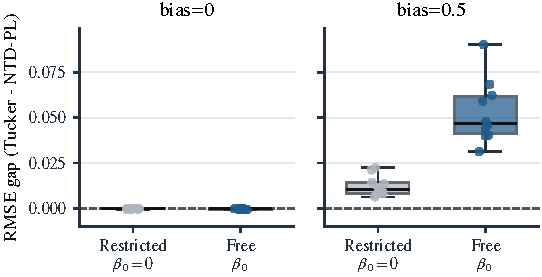
\includegraphics[width=\textwidth]{./inputs/figures/main/linear_consistency_paired_gap.pdf}
    \caption{Distribution of paired differences in the linear-consistency experiment. The figure compares the paired error gap between Tucker and NTD-PL across random seeds under different settings, supplementing the scene-wise mean conclusion in Table~\ref{tab:linear-consistency}. One can see that when \texttt{bias=0}, the paired differences between Tucker and NTD-PL without a constant term are concentrated near zero; when an affine bias is present, a more obvious systematic gap appears between Tucker and the model with restricted $\beta_0$.}
    \label{fig:linear-consistency-paired-gap}
\end{figure}

\begin{figure}[htbp]
    \centering
    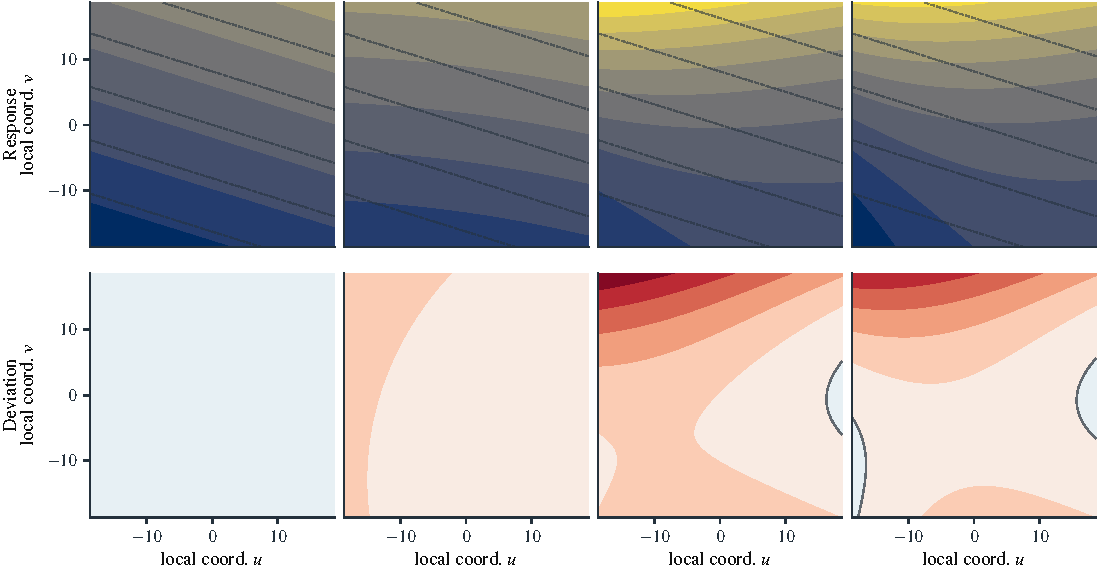
\includegraphics[width=\textwidth]{./inputs/figures/appendix/geometry_response_maps.pdf}
    \caption{Learned local response maps and deviation maps relative to $P=1$ under different maximum polynomial degrees $P$, for a fixed two-dimensional Tucker local patch. The top row shows the local responses, and the bottom row shows the deviations relative to the linear baseline.}
    \label{fig:geometry-response}
\end{figure}

\subsection{Supplementary Real Hyperspectral Experiments}

\begin{figure}[htbp]
    \centering
    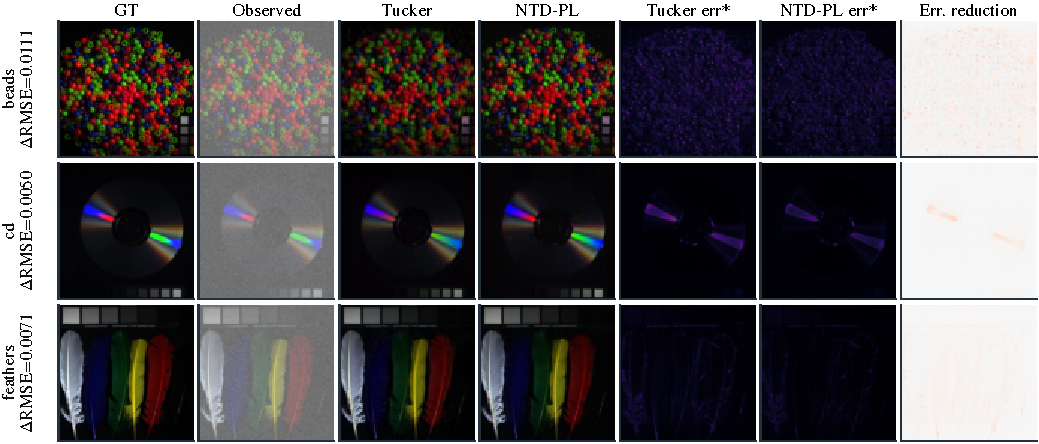
\includegraphics[width=\textwidth]{./inputs/figures/main/cave_completion_visual_grid.pdf}
    \caption{Representative spatial visualization of random-missing completion on CAVE. The columns show, in order, the original image, the masked observation input, Tucker completion, NTD-PL completion, the missing-only error of Tucker, the missing-only error of NTD-PL, and the missing-only error-reduction map. The last column is defined as Tucker $-$ NTD-PL, so positive values indicate that NTD-PL further reduces the completion error at the missing entries.}
    \label{fig:cave-completion-visual-app}
\end{figure}
